\subsection{Het web en HTTP}

\subsubsection{Overzicht van HTTP}

Het \textbf{\acrfull{http}}, de web applicatie laag protocol, is het centrum van het web. HTTP is geïmplementeerd in twee programma’s: een client en server programma. De client en server praten met elkaar door het uitwisselen van berichten.

\noindent HTTP gebruikt TCP als onderliggende transport protocol. 

\noindent De client initialiseert eerst een TCP connectie met de server. Eenmaal dat connectie gezet is, kunnen de browser en server processen de TCP bereiken door hun socket interfaces.

\noindent Berichten worden via de browser verstuurd.

\noindent Omdat een HTTP-server geen info over de clients bijhoudt m.b.t. eerder verzonden berichten, wordt HTTP een \textbf{toestandsloos} of \textbf{stateless protocol} genoemd.

\newpage

\subsubsection{Niet aanhoudende en aanhoudende connecties}

\subsubsubsection{HTTP met niet aanhoudende connecties}

Wanneer verzoeken en responsen via (verschillende) dezelfde TCP verbinding(en) lopen, noemt men deze verbinding (non-) \textbf{persistent}.

\noindent \textbf{NON-persistent}: gang van zaken (10 links op index.php naar een afbeelding)
\be
\itf Client maakt TCP-verbinding met server
\itf Client verzendt via zijn socket een HTTP-verzoekbericht met ‘/home/index.php’
\itf Server zoekt ‘/home/index.php’-object op, verpakt het in een HTTP-antwoordbericht en stuurt het naar de client.
\itf Server geeft opdracht aan TCP om de verbinding te verbreken (wanneer hij zeker weet dat het object is toegekomen)
\itf Client ontvangt bericht. Verbinding wordt gebroken. Client vindt 10 links naar de afbeeldingen op de index.php
\itf De eerste 4 stappen worden vervolgens herhaald voor elk van de 10 afbeeldingen.
\ee

\noindent \textbf{BELANGRIJK: ELKE TCP CONNECTIE VERZENDT EXACT 1 REQUEST MESSAGE EN 1 RESPONSE MESSAGE.}

\noindent De tijd die verstrijkt tussen het moment dat een client een verzoek doet om het bestand te ontvangen en het moment dat het wordt ontvangen heet de \textbf{\acrfull{rtt}}

\noindent Het RTT bevat pakket verspreiding vertragingen, pakket wachtrij vertraging in tussen routers en switches, en pakket verwerking vertragingen.

\noindent Een klik op een link zorgt voor het opstarten van een TCP connectie tussen de browser en server. Dit bevat een \textbf{three way handshake}. De client stuurt een klein TCP segment naar de server, de server erkent het en antwoord met een klein TCP segment en uiteindelijk erkent de client terug naar de server. De eerste twee stappen van de handshake nemen één RTT in beslag. Na de eerste twee delen, zend de client een HTTP request gecombineerd met het derde deel van de handshake. Eenmaal dat de request bericht aankomt, zend de server de HTML bestand door de TCP connectie. Deze HTTP request/response neemt nog een RTT in beslag. Dus de totale response tijd is twee RTTs plus de transitie tijd bij de server van de HTML bestand.

\newpage

\subsubsubsection{HTTP met aanhoudende connectie}

De server laat de TCP connectie open na het zenden van een response. Opeenvolgende requests en responses tussen dezelfde client en server kunnen over dezelfde connectie verzonden worden. Meer zelfs, meerdere web pagina’s die afkomstig zijn van één dezelfde server kunnen over die connectie gestuurd worden. Deze requests voor objecten kan back-to-back gemaakt worden, zonder te moeten wachten voor antwoorden op hangende requests. De HTTP server sluit een connectie wanneer het voor een bepaalde tijd niet meer gebruikt is.

\subsubsection{HTTP bericht formaat}

\subsubsubsection{HTTP request bericht = verzoekbericht}

\begin{figure}[h]
    \centering
    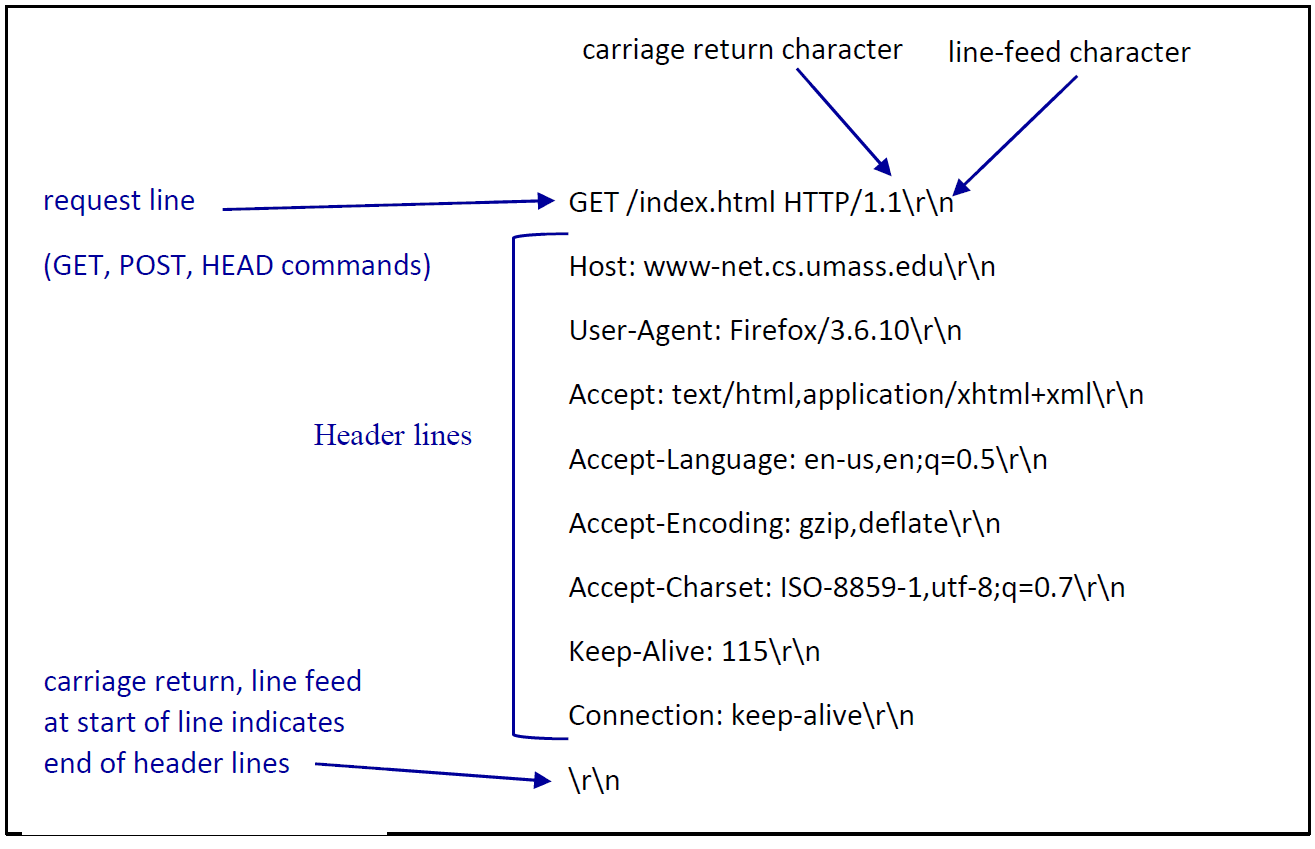
\includegraphics[width=7in]{./img/imghfdst2/httprequestmessage.PNG}
    \caption{Voorbeeld van een HTTP request message}
    \label{fig:http request message}
\end{figure}

\noindent Het bericht wordt in ASCII text geschreven zodat we het bericht kunnen lezen.

\noindent De request line heeft \textbf{drie velden}; de methode veld, de URL veld en de HTTP versie veld.

\noindent Het methode veld kan verschillende waardes aannemen zoals GET, POST, HEAD, PUT en DELETE.

\noindent Door Connection: toe te voegen, vertelt de browser tegen de server of de connectie open of gesloten moet blijven. 

\noindent De User-Agent: is handig omdat de server verschillende versies van het zelfde object kan sturen naar verschillende types van user agents.

\subsubsubsection{HTTP request message: general format}

\begin{figure}[h]
    \centering
    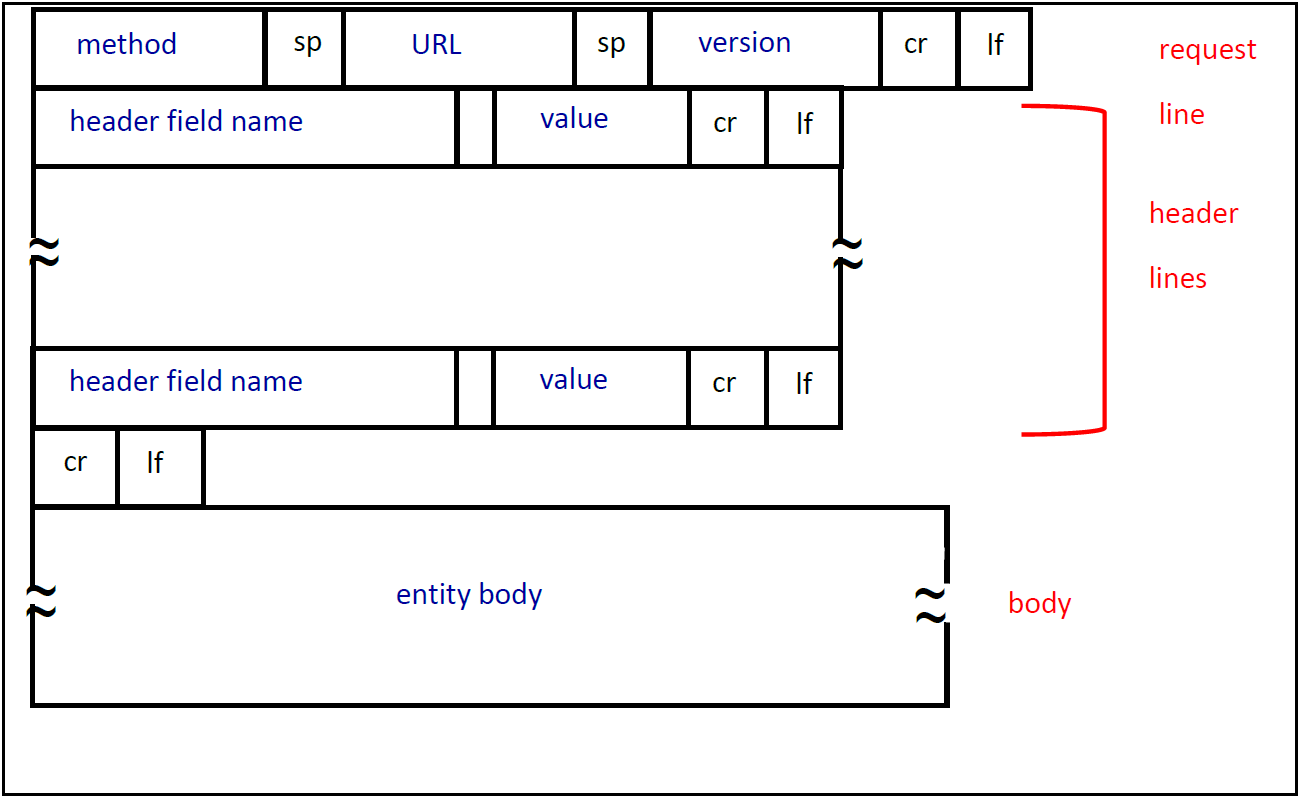
\includegraphics[width=7in]{./img/imghfdst2/httprequestgeneral.PNG}
    \caption{Voorbeeld van een HTTP request message format}
    \label{fig:http request message format}
\end{figure}

\newpage

\subsubsubsection{HTTP response bericht}

\begin{figure}[h]
    \centering
    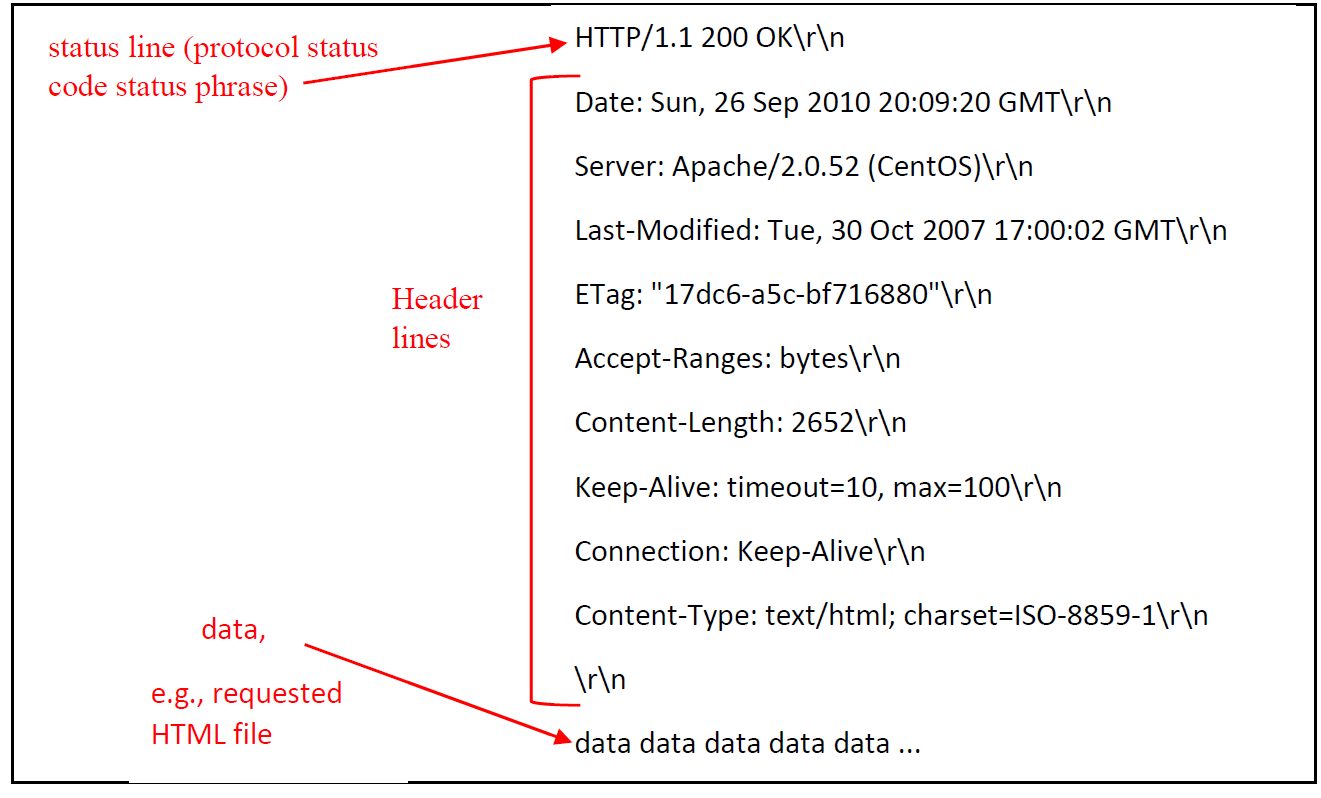
\includegraphics[width=7in]{./img/imghfdst2/httpresponse.PNG}
    \caption{Voorbeeld van een HTTP response message}
    \label{fig:httpresponse}
\end{figure}

\noindent Het heeft drie secties: een initiële status line, header lines en dan de entity body. De entity body bevat het gevraagde object. De status lijn heeft drie velden: het protocol versie veld, een status code, en een bijhorende status bericht.
De status code en bijhorende text duiden het resultaat van het request aan. Hier zijn een paar voorbeelden:
\begin{itemize}

 \item 200 OK: request is succesvol en de informatie is teruggezonden in de response.
 \item 301 Moved Permanently: de nieuwe URL wordt gespecificeerd in de Location: header van de response bericht. De client zal automatisch de nieuwe URL ophalen.
 \item 400 Bad Request: de request kon niet begrepen worden door de server.
 \item 404 Not Found: de gevraagde document bestaat niet op dit server.
 \item 505 HTTP Version Not Supported: de gevraagde HTTP protocol versie is niet ondersteund op de server.
\end{itemize}

\newpage

\subsubsection{Gebruiker-server interactie: Cookies}

\noindent \textbf{Cookie}: bestand dat wordt bijgehouden door de server waarin bepaalde gegevens staan opgeslagen i.v.m. met de gast op zijn webpagina.

\noindent \textbf{Nadeel}? Schending van privacy. Keuzes die gemaakt worden op websites worden opgeslagen in deze cookies en kunnen worden doorverkocht aan derden met doelgerichte reclame als gevolg.

\noindent Cookie-technologie heeft 4 componenten:
\be
\itf Een cookie header line in de HTTP response message
\itf Een cookie header line in de HTTP request message
\itf Een cookie-bestand opgeslagen op het systeem van de
eindgebruiker en beheerd door de webbrowser
\itf Een back-end database op de website
\ee

\noindent Voorbeeld:
\be
\itf Susan always access Internet from PC
\itf visits specific e-commerce site for first time
\itf when initial HTTP requests arrives at site, site creates:
\itf unique ID
\itf entry in backend database for ID
\ee

\begin{figure}[h]
    \centering
    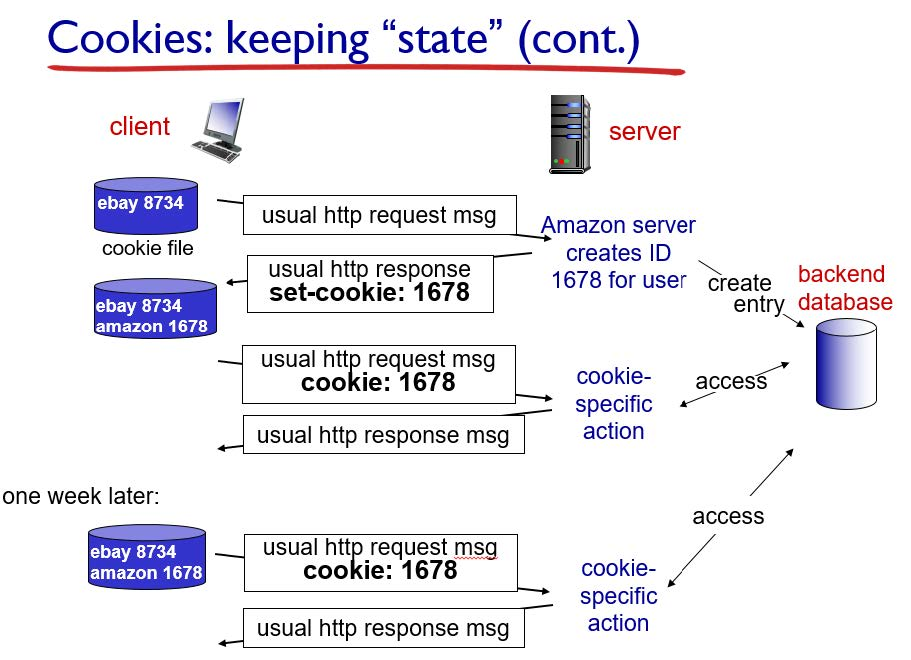
\includegraphics[width=4.5in]{./img/imghfdst2/cookie.jpg}
    \caption{Voorbeeld van een cookie }
    \label{fig:cookie}
\end{figure}

\newpage

\noindent Cookies kunnen dus gebruikt worden om een gebruikers sessie laag te maken bovenop de stateless HTTP. Cookies kunnen ook als controversieel opgevat worden omdat ze ook beschouwd worden als een inbreuk op de privacy. Zo kan een website veel leren van een gebruiker, en potentieel deze informatie verkopen.

\begin{multicols}{2}
\noindent \textit{\textbf{what cookies can be used for:}}

\bi
\itf authorization
\itf shopping carts
\itf recommendations
\itf user session state (Web e-mail)
\ei

\noindent How to keep "state"?

\bi
\itf protocol endpoints:

maintain state at sender/receiver

over multiple transactions
\itf cookies: http messages carry state
\ei
\end{multicols}


\subsubsection{Web caching}

\noindent \textbf{\gls{webcache}:} Een netwerkentiteit die HTTP-verzoeken afhandelt namens de oorspronkelijke webserver waar het verzoek oorspronkelijk naartoe is gestuurd.

\noindent Definition english: goal: satisfy client request without involving origin server

\noindent De web cache heeft zijn eigen schijf opslag en houdt kopieën bij van recent opgevraagde objecten. Een gebruiker zijn browser kan zo geconfigureerd zijn dat alle HTTP requests eerst naar de Web cache gaan. Als dit zo is, dan gebeurt het volgende:
\begin{enumerate}
    \item De browser zet een TCP connectie op met de Web cache en zend een HTTP request voor het object naar de web cache.
\item De web cache kijkt of er een kopie van dat object lokaal opgeslagen is. Als dit zo is, stuurt de cache het object terug binnen een HTTP response bericht naar de client.
\item Als de cache het object niet heeft, opent de cahce een TCP connectie naar de oorsprong server. De web cache zend een HTTP request voor het object. De oorsprong server zend het object binnen een HTTP response naar de web cache.
\item Wanneer de web cache het object krijgt, slaagt het een kopie op, en zend het een kopie door binnen een HTTP response bericht naar de client.
\end{enumerate}

\begin{figure}[h]
\centering
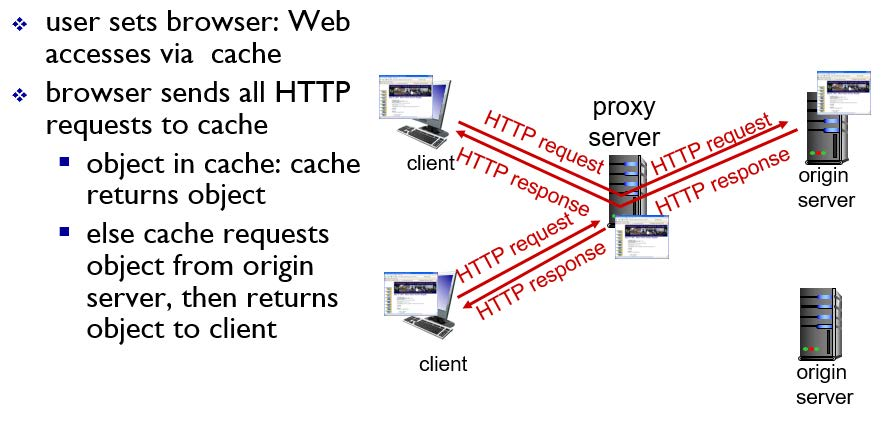
\includegraphics[width=4.5in]{./img/imghfdst2/webcache.jpg}
\caption{Voorbeeld van een webcache }
\label{fig:webcache}
\end{figure}

\newpage

\noindent Redenen:
\bi
\itf Kan responstijd van verzoeken aanzienlijk verkorten (omdat het is opgeslagen in de cache van de proxy)
\itf Men kan door de proxy te gebruiken (waarop kopieën staan van bepaalde webpagina’s) de bandbreedte die wordt verbruikt naar het internet versmallen = voordeliger.
\ei

\noindent Door het gebruik van Content Distribution Networks (CDNs), spelen web caches steeds een grotere rol. Een CDN bedrijf installeert veel geografisch verdeelde caches over het internet, om zo veel van het verkeer te lokaliseren.

\subsubsection{De conditionele GET}

\noindent \textbf{\Gls{conditionalget}}: Een GET-bericht dat de proxy naar de server stuurt om te achterhalen of het bestand dat in zijn cache staat al een oud bestand is of niet, dus of het cache een up-to-date versie heeft of niet.

\noindent \textbf{\gls{cache}}: specify date of cached copy in HTTP request

\noindent $\Rightarrow$ If-modified-since: $<date>$

\noindent \textbf{server}: response contains no object if cached copy is up-to-date:

\noindent $\Rightarrow$ HTTP/1.0 304 Not Modified
